\section{Grundlagen}
%Im Grundlagenkapitel stellen Sie das Basiswissen für die weiteren Kapitel vor. 
%Hierzu können neben theoretischen Konzepten auch die historische Entwicklung 
%und aktuelle Forschungsvorhaben gehören. Idealerweise bedient man sich hier 
%mehrerer verschiedener Quellen, um die Ausführungen zu belegen.

%Nachfolgend werden einige Formalitäten der Arbeit dargestellt.
\subsection{Cloud \-- Definitionen}
Das US-amerikanischen National Institute of Standard and 
Technology (NIST) von \pcite{}{}{NIST} definiert Cloud Computing als 
"`model for enabling ubiquitous, convenient, on-demand 
network access to a shared
pool of configurable computing resources [\dots] that
can be rapidly provisioned and released with minimal management effort or 
service provider interaction."' Das Model der Cloud unterteilt es in fünf 
Charakteristika, drei Service-Modelle und vier Deployment Modellen, die ich 
hier lediglich (ins Deutsche übersetzt) wiedergebe.
\subsubsection{Charakteristika}
\begin{description}
	\item[Selbstbedienung bei Bedarf:] Ein Nutzer kann ohne 
zwischenmenschliche Interaktion mit dem Provider die automatische Zuteilung von 
Rechenkapazitäten anstoßen.
	\item[Umfassender Zugriff über das Netzwerk:] Die Dienstleistung ist 
über das Netzwerk mit standardisierten Methoden von hetrogenenen Thin- oder 
Thick-Client-Plattformen abrufbar.
	\item[Geteilte Ressourcennutzung] Kunden eines Cloud-Anbieters teilen 
sich physische oder virtuelle Rechenleistung die dynamisch und bedarfsgerecht 
zugeteilt wird. Der Nutzer kann keinen Einfluss darauf nehmen, an welchem Ort 
genau die Daten gespeichert werden. Dies kann bedeuten, dass der Kunde nicht 
genau weiß auf welcher Festplatte in einem Rechenzentrum seine Daten liegen. 
Diese Ungewissheit kann sich aber auch auf Städte, Staaten oder Kontinente 
ausweiten.
	\item[Schnelle Anpassungsfähigkeit] Rechenkapazitäten können dem Bedarf 
entsprechend, teilweise automatisch, schnell zugewiesen und entzogen werden. 
Auf den Kunden wirkt die abrufbare Rechenleistung oftmals unbegrenzt.
	\item[Messbare Dienstleistung] Cloud Systeme messen und optimieren 
Ressourcennutzung automatisch und stellen die Auslastung sowohl dem Cloud 
Anbieter als auch dem Nutzer zur Verfügung.
\end{description}
\subsubsection{Service Modelle}
\begin{description}
	\item[Software as a Service (SaaS)] Der Kunde nutzt die Anwendungen des 
Anbieters die über verschiedene Geräte abrufbar
sind und in einer Cloud Infrastruktur liegen. Die Cloud Infrastruktur, 
bestehend aus Netzwerken, Servern, Betriebssystemen, Speichern und sonstigen 
anwendungsabhängigen Fähigkeiten, ist für den Kunden transparent; Details kann 
er weder sehen noch verändern.
	\item[Platform as a Service (PaaS)] Der Service-Anbieter stellt dem 
Kunden eine Cloud-Infrastruktur zur Verfügung auf der der Kunde eine selbst 
entwickelte Anwendung ausführen kann. Die zugrundeliegende Infrastruktur ist 
wie bei SaaS transparent. Anpassbar sind lediglich bestimmte, die 
Anwendungsausführung betreffende Optionen. 
	\item[Infrastructure as a Service (IaaS)] Der Anbieter stellt dem 
Kunden Rechenleistung, Speicher, 
Netzwerkkapazitäten und sonstige, grundlegende Computerressourcen zur 
Verfügung, auf der dieser beliebige Anwendungen bis hin zu Betriebssystemen 
auswählen kann. Der Kunde hat keinen Einfluss auf die tatsächlich 
bereitgestellte Hardware, kann jedoch auf Software-Seite einschließlich dem 
Betriebssystem alle Parameter selbst bestimmen.
\end{description}

\subsubsection{Deployment Modelle}
\begin{description}
	\item[Private Cloud] Die Cloud Infrastruktur steht nur einem einzigen 
Kunden zur Verfügung. Über den Ort der Leistungserbringung, 
Organisationsstruktur, sowie den Besitzer und Eigentümer wird dabei keine 
Aussage getroffen. Die Cloud kann beim Nutzer "`lokal"' oder bei einem anderen 
Cloud Anbieter betrieben werden.
	\item[Community Cloud] Im Gegensatz zur Private Cloud steht die 
Infrastruktur hier einer Gruppe ("`Community"') mit übereinstimmenden Zielen 
zur Verfügung.
	\item[Public Cloud] Die Nutzer der Cloud Infrastruktur kennen sich 
nicht. 
	\item[Hybrid Cloud] Die Cloud Infrastruktur besteht aus mindestens zwei 
der oben genannten Formen, die nicht verschmolzen werden, sondern über 
standardisierte Technologien Anwendungen und Daten austauschen.
\end{description}



\subsection{Herausforderungen in Migrationsprojekten als zu berücksichtigende 
Faktoren}
Um die Eignung einer Anwendung für eine Migration in die Cloud zu prüfen, 
schlagen \pcite{}{}{fivephases} die Berücksichtigung der folgenden der 
folgenden wirtschaftlichen und technischen Faktoren vor. Um diese Faktoren in 
einem geordneten Prozess zu berücksichtigen, führen sie ein Vorgehensmodell 
ein. Dieses Vorgehensmodell hat den Vorteil, dass es an bestehende Strukturen 
und Begrifflichkeiten anknüpft und sich deshalb besonders gut vergleichen, 
ergänzen und diskutieren lässt. Aus diesem Grund soll es den Rahmen dieser 
Arbeit bilden.

\subsubsection{Wirtschaftliche Faktoren}
\begin{description}
	\item[Bereits getätigte IT-Investitionen:]
	Je größer das Unternehmen, das eine Anwendung in die Cloud migrieren 
will, desto größer sind die bereits getätigten Investitionen in die 
IT-Infrastruktur. Mit den Investitionen steigt in der Regel auch die 
Komplexität, was eine Migration erschwert.
	\item[Kosten:] Älteren Unternehmen fällt es aufgrund der langjährigen 
Erfahrung leicht die Kosten für die bestehende Softwarelösung abzuschätzen. 
Kosten, die zudem bereits genehmigt und eingeplant sind. Dem stehen die 
nutzungsbezogenen, bisher unbekannten Kosten einer Cloudlösung gegenüber. Diese 
Kosten sollten über eine Prognose der benötigten Rechen-, Speicher- und 
Transferkapazitäten, den Betriebs-, Lizenz- und Migrationskosten abgeschätzt 
werden, damit erhoffte Kosteneinsparungen auch tatsächlich realisiert werden 
können.
	\item[Datensicherheit:] Für den Unternehmenserfolg kritische Daten sind 
auf unternehmenseigenen Servern eventuell besser aufgehoben.
	\item[Rechtliche Restriktionen:] Das Unternehmen könnte rechtlichen 
Rahmenbedingungen ausgesetzt sein, die eine Migration in die Cloud ausschließen.
	\item[Zuteilung von Rechenleistungen:] Anwendungen, die kurzzeitig 
große Rechenleistungen benötigen und gut skalierbar sein sollen, lassen sich in 
der Cloud wahrscheinlich kostengünstiger betreiben als auf Servern die 
ganzjährig reserviert sind und sind damit geeignetere Kandidaten für eine 
Migration.
\end{description}

\subsubsection{Technische Faktoren}
\begin{description}
	\item[Bestehende Infrastruktur:] Mit der Infrastruktur, die sich im 
Laufe einer Migration ändert, ändert sich auch die Art, wie Anwendungen an 
Endnutzer ausgeliefert werden. Auch der Support wird möglicherweise nach der 
Migration nicht mehr über den IT-Support im Haus abgewickelt, sondern über den 
Cloud-Anbieter. 
	\item[Sicherheitsarchitektur:] Um die Daten im Cloud-Umfeld zu 
schützen, muss das bestehende Sicherheitskonzept an die Gegebenheiten der Cloud 
angepasst werden.
	\item[Komplexität:]
	Während einfache Anwendungen womöglich bereits in der Cloud angeboten 
werden, steigt mit der Komplexität auch der Planungs-, Implementierungs- 
und Testbedarf bei der Migration.
	\item[Netzwerk und Support:] Je mehr Daten in der Cloud liegen, desto 
höher ist die Abhängigkeit von einer funktionierenden Internetverbindung. Hier 
können zusätzliche Kosten für Verbindungen mit höheren Kapazitäten oder 
Verträge mit garantierten Reaktionszeiten im Störungsfall anfallen. Bei der 
Bewertung dieses Faktors schlage ich vor, die bereits vorhandene Abhängigkeit 
als Referenz zu nutzen. 
	\item[IT-Fähigkeiten:] Die Migration in die Cloud fordert dem IT-Team 
andere Fähigkeiten ab, als der lokale Betrieb und ist daher mit einer steileren 
Lernkurve verbunden. Sie geht außerdem regelmäßig mit einem Gefühl des 
Kontrollverlustes einher. 
	\item[Service Level Agreements (SLAs):] Geprüft werden sollte auch, ob 
Cloud-Anbieter SLAs bieten können, die zum unternehmerischen Bedarf 
hinsichtlich Verfügbarkeit, Vertraulichkeit und Integrität passen. Auch sollte 
geregelt sein, welche Verantwortlichkeiten der Anbieter trägt und welche 
Strafen bei Nichteinhaltung drohen.
\end{description}

\subsection{Das Fünf-Phasen-Wasserfallmodell}
Das in \citepara{fivephases} vorgeschlagene Vorgehensmodell ähnelt dem aus der 
Softwareentwicklung bekannten, klassischen Wasserfallmodell und besteht aus den 
folgenden fünf Phasen, die in Abbildung 
\ref{fuenf-phasen-wasserfall-modell}
dargestellt sind.
\begin{figure}[h]
\begin{center}
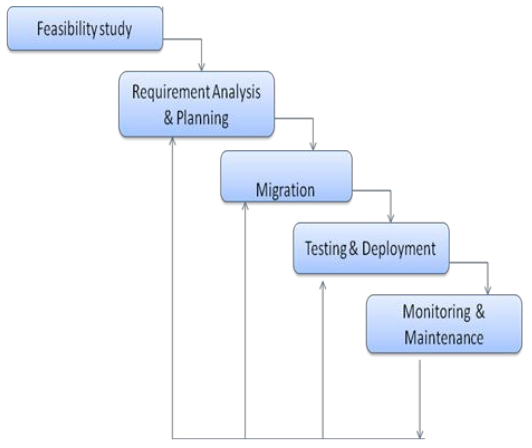
\includegraphics[width=0.6\textwidth]{images/fuenf-phasen-wasserfall-modell.png}
\caption{Das Fünf-Phasen-Wasserfallmodell aus \protect\citeflow{fivephases} }
\label{fuenf-phasen-wasserfall-modell}
\end{center}
\end{figure}
\begin{enumerate}
	\item Die technische und wirtschaftliche \textbf{Machbarkeitsstudie}
analysiert die bestehende Anwendung in Hinblick auf Dateneingabe, 
Datenverarbeitung, Datenausgabe und sonstige Randbedingungen und Erwartungen. 
Das Ergebnis der Machtbarkeitsstudie ist eine detaillierte  
Kosten-Nutzen-Analyse. Als Grundlage einer wirtschaftlich vernünftigen 
Migrationsentscheidung muss sie ergebnisoffen verlaufen.
	\item Die \textbf{Anforderungsanalyse und -Planung} konkretisiert die 
Ergebnisse der Machtbarkeitsstudie weiter, indem sie die oben genannten 
wirtschaftlichen und technischen Faktoren berücksichtigt. Außerdem wird der 
Return on Investment sowie die Total Cost of Ownership berechnet.
	\item Mit der \textbf{Migration} ist nicht nur die Entwicklung 
beziehungsweise Einrichtung der Cloudsoftware gemeint, sie enthält auch Tests 
der Funktionalität, Performanz und Nutzerakzeptanz.
	\item Beim \textbf{Ausrollen (Go-Live) und Testen} wird die 
Cloud-Anwendung mit den Betriebsdaten ausführlich getestet und 
schließlich freigegeben. Die Freigabe ist mit intensiver Beobachtung und 
verstärktem Support zu begleiten um auftretenden Problemen begegnen zu können. 
Je nach Größe, Relevanz und Art der Anwendung ist zu prüfen, ob in der 
Anfangsphase  ein paralleler Ansatz gewählt wird, bei dem die bestehende Lösung 
weiter genutzt wird.
	\item Naturgemäß ist man bei Nutzung der Cloud bei Performanz, 
Verfügbarkeit und Sicherheit vom Anbieter abhängig. Die Einhaltung garantierter 
Leistungen und Erwartungen sollte man \textbf{überwachen}. Abweichungen lassen 
sich Idealerweise  \textbf{Wartungsarbeiten} an der Anwendung oder durch 
Einforderung von Leistungen beim Anbieter beheben.
\end{enumerate}
\subsubsection{Organisationsform als Einflussfaktor}
\citeflow{fivephases} identifizieren die Organisationsstruktur, beziehungsweise 
deren Größe und Komplexität und insbesondere drei Formen als 
wesentliche Einflussfaktoren für dieses Vorgehensmodell. Zu diesem Ergebnis 
kommen auch \citeflow{Pahl2013}.
\begin{description}
	\item[Große Unternehmen] haben gewachsene, komplexe IT-Strukturen, die 
umso detailliertere Analysen der Cloud-Eignung einzelner Anwendungen 
erforderlich machen und eine Schrittweise Migration nahelegen, bei der 
zunächst einfache Standardanwendungen wie E-Mail-Anwendungen migriert werden. 
Komplexe Anwendungen folgen sobald Erfahrungen im Cloud-Umfeld gesammelt wurden 
und gegebenenfalls fertige Anwendungen in der Cloud bereits existieren.
	\item[Kleinere und mittlere Unternehmen] haben gegenüber großen 
Unternehmen nicht nur den Vorteil einer kleineren, weniger komplexen 
IT-Landschaft. Bestehende Unternehmensprozesse lassen sich auch leichter an die 
Cloud-Nutzung anpassen, sodass sich viele bereits in der Cloud existierende 
Cloud-Anwendungen als SaaS nutzen lassen. Durch die nutzungsabhängige 
Bepreisung lassen sich in der Cloud möglicherweise Anwendungen nutzen, die 
bisher zu teuer oder zu komplex waren. Die nutzungsabhängige Bezahlung birgt 
allerdings wie bereits geschildert auch Risiken, die neben den anderen Faktoren 
ebenfalls vor der Migrationsentscheidung berücksichtigt werden sollten.
	\item[Regierungsorganisationen] dürften regelmäßig zwei Spezifika 
aufweisen, die bei der Prüfung der Cloud-Eignung einer Anwendung zu prüfen 
sind. Erstens sind sie in besonderem Maße, teilweise durch Gesetze, zur 
Kontrolle über die eigenen Daten und Funktionsfähigkeit ihrer Anwendungen 
gezwungen. Zweitens übersteigt die orts-, amts- oder ministerienübergreifende 
Zusammenarbeit die Komplexität von großen Unternehmen bei weitem. 
\end{description}



\subsection{Methoden zur Anforderungsermittlung in Migrationsprojekten}
\subsection{Aktuelle und prognostizierte Ressourcennutzung}
\subsection{Auswahl des Migrationsziels in der Cloud}
\subsection{Kostenabschätzung der Cloud-Lösung}

\newpage
\subsection{Abbildungen}

\begin{figure}[h]
\begin{center}

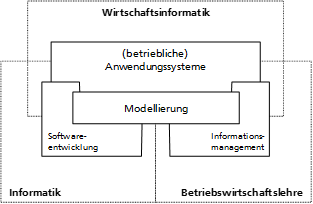
\includegraphics[width=10cm]{images/Abb2_3.png}
\caption{Einordnung der Wirtschaftsinformatik (angelehnt an Fink et al. 2001)}
\label{Abbildung2_3}
\end{center}
\end{figure}
Bitte achten Sie darauf, dass alle vorhandenen Abbildungen und Tabellen in einem inhaltlichen Zusammenhang mit dem Text stehen und Sie auf die entsprechende Abbildung (bspw. Abbildung 1) verweisen.
\subsection{Tabellen}
%hier Tabelle einfügen
\begin{table}[h]
\centering
\begin{tabular}{ccc}
\hline \textbf{Attribute} &\textbf{Typ}  & \textbf{1. Ausprägung (Beispiel)} \\ 
\hline Titel & \textit{STRING}& Aktiengesetz (AktG)  \\ 
Text& \textit{STRING} &  [Text des AktG]\\ 
Gültig von & \textit{DATE} & 01.01.2010 \\ 
Gültig bis & \textit{DATE} & - \\ 
Dok.-Besitzer & \textit{STRING} & Rechtsabteilung \\ 
Quelle & \textit{STRING}  & Deutsche Gesetze \\ 
Verplichtungsgrad & \textit{STRING} & verplichtend \\ 
\hline 
\end{tabular} 
\caption{Attribute der Anforderungsquellen im Metamodell}
\label{tab:tabelle 1}
\end{table}
\par\medskip

Tabelle 1 stellt eine beispielhafte Tabelle dar